\documentclass{iaf}

\annee{2015}


\usepackage[pdftex]{graphicx}
\usepackage{todonotes}
%\usepackage[colorlinks,hyperindex,bookmarks,linkcolor=blue,citecolor=blue,urlcolor=blue]{hyperref}
\usepackage{url}
%%%%%%%%%

\usepackage[normalem]{ulem} % for strikethrough in Latex
\usepackage{amssymb,amsmath}
\usepackage{xspace}

\pagestyle{plain}

\newcommand{\secref}[1]{Section~\ref{#1}}
\newcommand{\secrefs}[1]{Sections~\ref{#1}}
\newcommand{\figref}[1]{Figure~\ref{#1}}
\newcommand{\figrefs}[1]{Figures~\ref{#1}}

%\usepackage{color}
%\newcommand{\red}[1]{{\color{red}#1}}
%\newcommand{\green}[1]{{\color{green}#1}}
%\newcommand{\blue}[1]{{\color{blue}#1}}

% \newcommand{\remfs}[2][]{}
% \newcommand{\remog}[2][]{}
% \newcommand{\remms}[2][]{}
% \newcommand{\dremfs}[2][]{}
% \newcommand{\dremog}[2][]{}
% \newcommand{\dremms}[2][]{}
% \newcommand{\elimstart}[1][]{}
% \newcommand{\elimend}[1][]{}

\newcommand{\remfs}[2][]{\todo[color=blue!40,#1]{FS: #2}}
\newcommand{\remog}[2][]{\todo[color=red!40,#1]{OG: #2}}
\newcommand{\remms}[2][]{\todo[color=green!40,#1]{MS: #2}}

\newcommand{\dremfs}[2][]{\todo[color=red!10,bordercolor=white,nolist,#1]{FS: #2}}
\newcommand{\dremog}[2][]{\todo[color=blue!10,bordercolor=white,nolist,#1]{OG:
    #2}}
\newcommand{\dremms}[2][]{\todo[color=green!10,bordercolor=white,nolist,#1]{MS: #2}}

\newcommand{\elimstart}[1][]{\todo[color=yellow!70,nolist]{Start del: #1}}
\newcommand{\elimend}[1][]{\todo[color=yellow!70,nolist]{End del: #1}}

%\newcommand{\rem}[1]{\textbf{{\red{#1}}}}
%\newcommand{\remms}[1]{\textbf{{\green{MS: #1}}}}
%\newcommand{\remmg}[1]{\textbf{{\blue{MG: #1}}}}

\newcommand{\ie}{\emph{i.\,e.}~}
\newcommand{\eg}{\emph{e.\,g.}~}
\newcommand{\cf}{\emph{c.\,f.}~}

% Logique
\newcommand{\IMPL}[0]{\longrightarrow}
\newcommand{\IMPLL}[0]{\Longrightarrow} % another implication, to make
                                % a difference with reduction relations
\newcommand{\AND}[0]{\wedge}
\newcommand{\OR}[0]{\vee}
\newcommand{\NOT}[0]{\neg}
\newcommand{\FALSE}[0]{\perp}
\newcommand{\TRUE}[0]{\top}
\newcommand{\IFF}[0]{\leftrightarrow}
\newcommand{\ufb}[0]{\mbox{$\stackrel{?}{=}$}} % unifiable


%\newcommand{\panda}{{\sc Panda}}
\newcommand{\satoulouse}{{\sc Satoulouse}\xspace}

\newcommand{\keywords}[1]{\par\addvspace\baselineskip
\noindent\keywordname\enspace\ignorespaces#1}

\newcommand{\set}[1]{\{#1\}}

\newcommand{\atL}[2]{{\Large \geqslant}_{#1}^{#2}}
\newcommand{\atM}[2]{{\Large \leqslant}_{#1}^{#2}}
\newcommand{\exact}[2]{{\Large \#}_{#1}^{#2}}

\renewcommand{\satoulouse}{{\sc \texttt {SAToulouse}}}

\newcommand{\nameTool}{{\sc \texttt {TouIST}}}
%%%%%%%%%%



%\titre{Twist your logic with \nameTool\\
%\small (and easily formalize and solve real-world sized problems)}
\titre{La logique facile avec \nameTool\\
%\titre{Mod\'elisation logique et r\'esolution de probl\`emes combinatoires complexes avec \nameTool\\
\small (formalisez et r\'{e}solvez facilement des probl\`{e}mes du monde r\'{e}el)}

\auteurs{\textbf{Skander Ben Slimane$^2$, Alexis Comte$^2$, Olivier Gasquet$^{1\ 2}$, Abdelwahab Heba$^2$,}\\[1ex]
\textbf{Olivier Lezaud$^2$, Fr{\'e}d{\'e}ric Maris$^{1\ 2}$, Ma{\"e}l Valais$^2$}} 
%\auteurs{K.S. Ben Slimane \and A. Comte \and O. Gasquet
%\and A. Heba \and O. Lezaud \and F. Maris \and M. Valais} 

\institutions{
$^1$IRIT (Institut de Recherche en Informatique de Toulouse)\\
$^2$Universit{\'e} Paul Sabatier\\ Toulouse, France}

\mels{\{gasquet,maris@irit.fr\}}

\begin{document}
\creationEntete

\begin{resume}
Les solveurs SAT sont des outils puissants pour r\'{e}soudre des probl\`{e}mes logiques de taille r\'eelle, mais leur utilisation n\'{e}cessite des connaissances solides. Elle peut \^{e}tre vue par rapport \`a la logique comme l'utilisation d'un langage d'assemblage par rapport \`a la programmation. Il manque un langage de haut niveau pour permettre \`a des utilisateurs divers de tirer facilement profit de ces outils. \nameTool\ vise \`a combler cette lacune.
Il est d\'edi\'e \`a la logique propositionnelle et ses principales fonctions sont (1) d'offrir un langage logique de haut niveau pour exprimer succictement des formules complexes (par exemple des formules d\'ecrivant les r\`egles du Sudoku, des probl\`emes de planification\ldots) et (2) de trouver des mod\`eles \`a ces formules en utilisant un solveur ad\'equat et performant, que l'utilisateur n'a pas besoin de conna\^{i}tre.
Il consiste en une interface conviviale qui propose plusieurs facilit\'es syntaxiques et qui fait appel \`a des solveurs suffisamment puissants pour permettre de r\'esoudre automatiquement de grandes instances de probl\`emes difficiles (emplois du temps, Sudokus\ldots). Il peut interagir avec diff\'erents d\'emonstrateurs: solveurs SAT pur mais \'egalement solveurs SMT (SAT modulo th\'eories - comme la th\'eorie lin\'eaire sur les r\'eels, etc). Il peut donc \^{e}tre utilis\'e aussi bien par des d\'ebutants pour  des probl\`emes purement propositionnels, que par des \'etudiants de cycles sup\'erieurs ou m\^{e}me des chercheurs et ing\'enieurs, par exemple pour r\'esoudre des probl\`emes de planification impliquant de grands ensembles d'actions et des contraintes num\'eriques.
\end{resume}






%----------------------------------------------------------------------
\section{Historique}\label{sec:introduction}
%----------------------------------------------------------------------

O. Gasquet et F. Maris enseignent \`a l'Universit\'e Paul Sabatier \`a Toulouse. Ils enseignent la logique \`a diff\'erents niveaux, en d\'{e}marrant des cours d'introduction \`a la logique propositionnelle, jusqu'\`a des sujets avanc\'es pour les \'etudiants en Master, comme la logique modale ou la planification bas\'ee sur la logique. S. Ben Slimane, A. Comte, A. Heba, O. Lezaud et M. Valais sont des \'etudiants en Master de la m\^eme universit\'e. Ils ont mis en oeuvre \nameTool\ durant les trois mois de leur projet de Master.

\subsubsection*{Motivation des \'etudiants}
Au d\'ebut des \'etudes de premier cycle, nous (enseignants) avons constat\'e que la motivation des \'etudiants peut \^etre am\'elior\'ee en leur montrant que la logique est tr\`es utile pour les informaticiens et que l'informatique ne consite pas seulement \`a \'ecrire du code C ou Java. Classiquement, la logique est motiv\'ee par des exemples abstraits ou, au mieux, par des exemples ludiques. A un moment, nous avons pens\'e qu'il serait pr\'ef\'erable de leur montrer et pas seulement de leur dire qu'avec un peu de connaissance, la logique peut \^etre utilis\'ee pour r\'esoudre des probl\`emes difficiles que la taille emp\^eche de r\'esoudre facilement \`a la main ou exigerait une programmation assez complexe en C ou tout autre langage de programmation. \\

\subsubsection*{Gen\`ese de \satoulouse}

Lors de la conf\'erence ICTTL'2011, nous avions pr\'esent\'e \satoulouse\ \cite{GaScSt2011}, d\'edi\'e \`a la logique propositionnelle, dont les principales fonctions \'etaient (1) d'offrir un langage logique de haut niveau pour exprimer succictement des formules complexes et (2) de trouver des mod\`eles \`a ces formules en utilisant un solveur SAT performant.
%\satoulouse\ avait plusieurs inconv\'enients \`{a} corriger.

Bien s\^ur, il existe de nombreux outils logiques comme des prouveurs, assistants de preuves, \'editeurs de tables de v\'erit\'e\ldots sur Internet, m\^eme PROLOG aurait pu \^etre utilis\'e, mais aucun ne correspond \`a nos exigences qui sont :
\begin{itemize}
\item l'outil doit \^etre tr\`es facile \`a installer et \`a utiliser, sans syntaxe complexe ;
\item le prouveur peut \^etre utilis\'e comme une bo\^ite noire sans savoir comment il fonctionne ;
\item  aucune mise en forme normale,  aucun ordonnancement de clauses, ou aucune coupure PROLOG ne doivent \^etre requis ;
\item seulement une petite connaissance en logique devrait \^etre n\'ecessaire.
\end{itemize} 

Comme nous ne pouvions pas trouver un outil existant satisfaisant ces exigences, en 2010, nous avons commenc\'e \`a d\'evelopper le n\^otre, et nous sommes arriv\'es \`a l'id\'ee de d\'evelopper simplement une interface qui permet d'utiliser tr\`es confortablement un prouveur SAT (\`a savoir SAT4J \cite{DBLP:journals/jsat/BerreP10}) : cet outil avait \'et\'e applel\'e \satoulouse\ et est d\'ecrit dans \cite{GaScSt2011}. Avec cet outil, les \'etudiants pouvaient exp\'erimenter par eux-m\^eme qu'un langage logique n'est pas seulement descriptif mais peut conduire \`a des calculs qui r\'esolvent des probl\`emes de la vie r\'eelle. En particulier, avec \satoulouse, ils pouvaient r\'esoudre des Sudokus assez facilement, ainsi que beaucoup d'autres probl\`emes combinatoires (emplois du temps, coloration de carte, circuits \'electroniques\ldots).\

Voici les principales facilit\'es qu'offraient \satoulouse\ :
\begin{itemize}
\item les formules entr\'ees n'ont pas besoin d'\^etre sous forme clausale et des connecteurs arbitraires peuvent \^etre utilis\'es, la mise sous forme normale est faite dynamiquement pendant la saisie au clavier de l'utilisateur ;
\item des facilit\'es d'utilisation de grandes conjonctions ou disjonctions sont offertes comme dans :
\end{itemize}
  \[\bigwedge_{i\in\{1..9\}}
  \bigvee_{j\in\{1..9\}}\bigwedge_{n\in\{1..9\}}\bigwedge_{m\in\{1..9\},m\neq
    n}(p_{i,j,n}\rightarrow \lnot p_{i,j,m})\]
\begin{itemize}
\item d\'emarrer le solveur consiste \`a cliquer sur un bouton ;
\item l'outil affiche un mod\`ele dans la syntaxe de la formule entr\'ee.
\end{itemize}
Ainsi, il est possible de montrer la puissance de la logique propositionnelle \`a des \'etudiants qui ont \'et\'e form\'es quelques heures \`a la formalisation de phrases en logique et qui ont acquis les notions de bases de validit\'e et satisfiabilit\'e pour r\'esoudre automatiquement des Sudokus.\

 
\subsubsection*{Travaux pratiques avec \satoulouse}
Mais ce n'est pas toute l'histoire, puisque le m\^eme solveur SAT peut \^etre utilis\'e pour r\'esoudre de nombreux autres probl\`emes combinatoires aussi facilement que pour le Sudoku : ils suffit juste de formaliser les contraintes.\ Nos \'etudiants sont invit\'es \`a le faire pour : des emplois du temps, des colorations de cartes,\ldots \satoulouse\ a \'et\'e utilis\'e pendant trois ans par environ 400 \'etudiants avec une grande satisfaction. En particulier, les \'etudiants l'ont utilis\'e pour effectuer des devoirs \`a long terme dans l'esprit de la programmation de projets : nous leur donnons un probl\`eme logique \`a r\'esoudre (trop gros pour \^etre r\'esolu \`a la main), ils doivent le formaliser et ensuite utiliser cette formalisation pour le r\'esoudre. Par exemple, un probl\`eme de stockage de produits chimiques qui doivent \^etre stock\'es dans des salles identiques/contig\"ues/non-contig\"ues en fonction de leur degr\'e de compatibilit\'e. Les \'etudiants doivent r\'esoudre un cas impliquant beaucoup de produits chimiques.


\subsubsection*{Limites de \satoulouse\ et gen\`ese de \nameTool}
Mais pendant ces ann\'ees, nous avons remarqu\'e quelques limitations dommageables de \satoulouse\ : de nombreux bugs, des d\'efauts dans l'interface, le manque de modularit\'e (si l'on souhaite changer le prouveur SAT utilis\'e), l'ambigu\"it\'e et les limites de son langage, etc.

Par exemple, des probl\`{e}mes impliquant des contraintes de cardinalit\'{e}, comme les r\`{e}gles du jeu de Takuzu\footnote{Connu aussi sous le nom de Binero.\\ \url{http://fr.wikipedia.org/wiki/Takuzu}} qui n\'{e}cessitent de compter des 0 et des 1, ne peuvent \^{e}tre facilement formalis\'{e}s : il manque des fonctionnalit\'{e}s permettant d'exprimer des choses comme ``exactement 5 parmi 10 propositions sont vraies''. 

De plus, \satoulouse\ n'offre pas la possibilit\'{e} de parcourir l'ensemble des mod\`{e}les fournis par le solveur, il en retourne seulement un.

Les le\c cons tir\'{e}es de trois ann\'{e}es d'utilisation de \satoulouse\ sont que beaucoup de nos \'{e}tudiants en informatique ont clairement pris conscience que la logique avait des applications r\'{e}elles en ce qui concerne la r\'{e}solution de probl\`{e}mes, et beaucoup d'entre-eux ont acquis une capacit\'{e} dans la formalisation de probl\`{e}mes. Mais les d\'{e}fauts de \satoulouse\ rendent le d\'{e}bogage vraiment difficile, d'une part parce qu'un seul mod\`{e}le est affich\'{e} et en raison de la fa\c con dont ce mod\`{e}le est affich\'{e}, et d'autre part \`a cause des faibles capacit\'{e}s d'\'{e}dition dont il dispose. En outre, seuls des probl\`{e}mes combinatoires purs peuvent \^{e}tre trait\'{e}s, ce qui limite lourdement la pr\'{e}tention de r\'{e}solution d'une large gamme de probl\`emes par \satoulouse\ concernant les probl\`{e}mes du monde r\'{e}el.

Un autre inconv\'{e}nient de \satoulouse , pas n\'{e}cessairement li\'{e} \`{a} l'enseignement de la logique, est son incapacit\'{e} \`{a} \^{e}tre utilis\'{e} \`{a} partir de la ligne de commande : des chercheurs ou des ing\'{e}nieurs qui souhaiteraient l'utiliser intensivement trouveraient fastidieux de taper des probl\`{e}mes en entr\'{e}e.

Enfin, l'extension \`{a} des th\'{e}ories plus riches est \'egalement quelque-chose qui peut int\'{e}resser les chercheurs, les ing\'{e}nieurs ou les \'{e}tudiants de cycles sup\'{e}rieurs. \satoulouse\ n'est certainement pas adapt\'{e} pour la satisfiabilit\'{e} modulo th\'{e}ories ou pour r\'{e}soudre des probl\`{e}mes de planification alors que la m\^{e}me architecture logicielle pourrait \^{e}tre utilis\'ee en changeant juste le solveur.


Il y a quelques mois, nous avons commenc\'{e} \`{a} d\'{e}velopper un nouveau logiciel qui comblerait ces lacunes et remplirait nos attentes. Nous l'avons appel\'e \nameTool\ qui signifie TOUlouse Integrated Satisfiability Tool et doit \^etre prononc\'e ``twist''.
 \nameTool\ est bien s\^ur \`a la disposition du public pour t\'el\'echargement \`a partir du site suivant :
\begin{center}\url{ https://github.com/olzd/touist/releases }\end{center}


Pour r\'{e}sumer, voici quelques fonctionnalit\'{e}s offertes par \nameTool\ et que \satoulouse\ ne propose pas :
\begin{itemize}
\item d\'{e}finition d'ensembles de domaines : $\bigwedge_{i\in A}$ vs. $\bigwedge_{i\in\{Paris,London,Roma,Madrid\}}$
\item liaisons multiples sur les indices: $\bigwedge_{i\in A,j\in B}$ vs. $\bigwedge_{i\in \cdots} \bigwedge_{j\in \cdots}$
\item calculs riches sur les indices ainsi que sur les ensembles de domaines: $\bigwedge_{i\in (A\cup (B \cap C))}$
\item primitives de contraintes de cardinalit\'{e} int\'{e}gr\'{e}es: ``auMoins'' (resp. ``auPlus'', ``exactement'') \emph{tant} de valeurs sont vraies parmi \emph{ces valeurs}
\item les pr\'{e}dicats peuvent \'{e}galement \^{e}tre des variables d\'{e}finies sur des ensembles de domaines: $\bigwedge_{X\in \{A,B\},i\in \{1,2\}} X(i)$ vs. $\bigwedge_{i\in \{1,2\}} (A(i)\AND B(i))$
\item litt\'{e}raux sp\'{e}ciaux d\'{e}finissant des contraintes entre nombres entiers ou r\'{e}els : ($x+y\leq z$)
\item parcours facile des mod\`{e}les successivement calcul\'{e}s par les solveurs
\item expressions r\'{e}guli\`{e}res permettant un filtrage des litt\'{e}raux pertinents
\item possibilit\'{e} d'utiliser le logiciel en ligne de commande et/ou batch
\item nombreuses fonctionnalit\'{e}s d'\'{e}dition et am\'{e}liorations
\end{itemize}







%......................................................................
\section{Vue d'ensemble de \nameTool}\label{sec:sat_interface}
%......................................................................


\nameTool\ est compos\'e de trois modules, mais l'utilisateur standard ne verra que l'un d'entre eux : l'interface. Dans la suite nous insistons principalement sur cette derni\`ere plut\^ot que sur le traducteur et le solveur. L'architecture globale est illustr\'{e}e par la figure~\ref{fig:architectureTouisT}: 

\begin{figure}[htbp]
\centering
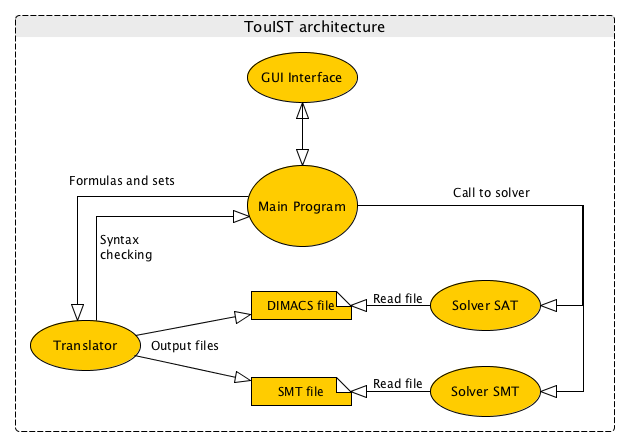
\includegraphics[scale=0.37]{DiagTouist.png}
  \caption{Architecture de TouIST}
  \label{fig:architectureTouisT}
\end{figure}

Avec \nameTool\ on acc\`ede \`a un \'editeur puissant et convivial pour \'editer des formules logiques complexes et des contraintes vari\'ees comme :

$$\bigwedge_{i \in \{1..9\}} (P_i \IMPL Q_{i+1})$$

qui abr\`ege confortablement :\\ 

$(P_1 \IMPL Q_2) \AND (P_2 \IMPL Q_3) \AND \ldots (P_9\IMPL Q_{10})$. 
\\

Une fois qu'un ensemble de formules a \'et\'e donn\'e \`a l'interface, sa satisfiabilit\'e peut \^etre v\'erifi\'ee : l'interface peut l'envoyer au prouveur qui retourne un mod\`ele, affich\'{e} comme le montre la figure \ref{fig:ExampleOfAModel} si un tel mod\`{e}le existe. Ensuite par l'interm\'ediaire de l'interface, l'utilisateur peut par exemple demander d'autres mod\`eles (bouton ``Next'' de l'interface). Contrairement \`a \satoulouse\ qui aurait n\'ecessit\'e de modifier les formules pour interdire le mod\`ele et de relancer le solveur, \nameTool\ conserve une instance du solveur en attente, ce qui permet d'obtenir les mod\`eles suivants bien plus rapidement.

\begin{figure}[htbp]
\centering
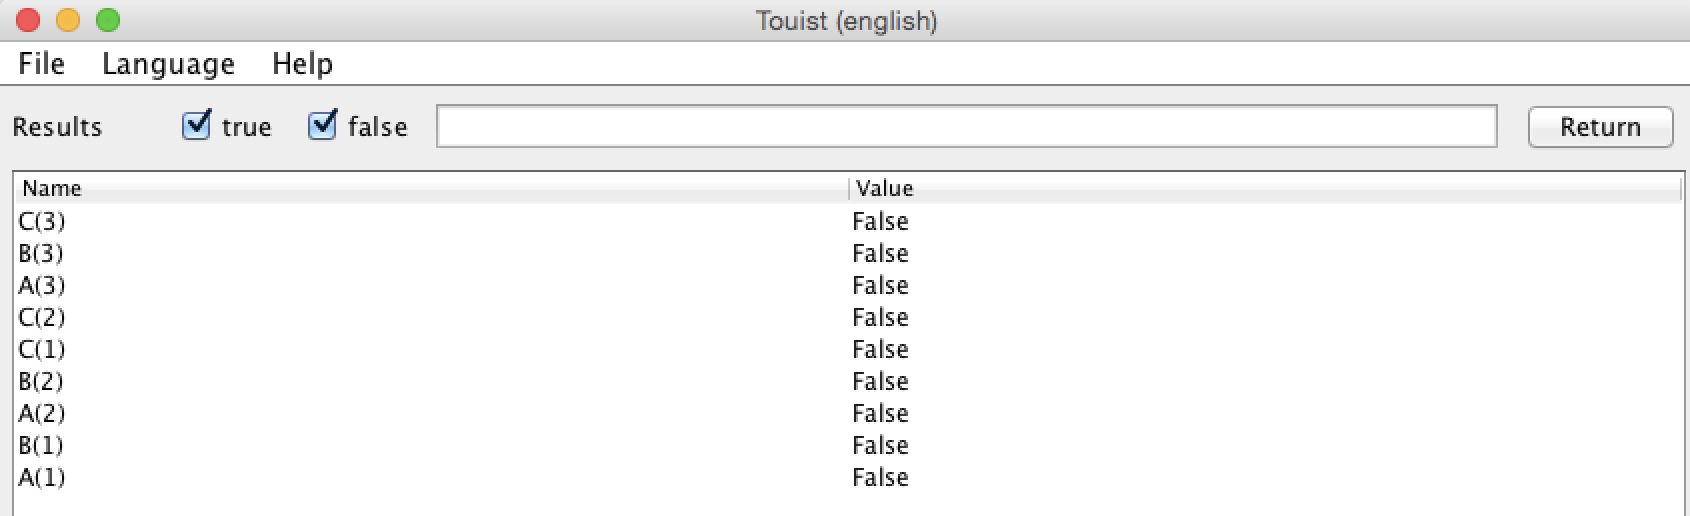
\includegraphics[scale=0.27]{ExampleOfAModel.png}
  \caption{Affichage de mod\`{e}le}
  \label{fig:ExampleOfAModel}
\end{figure}

Les mod\`{e}les renvoy\'{e}s par le solveur sont totaux : une valeur est affect\'{e}e \`{a} chacune des variables apparaissant dans les formules envoy\'{e}es au solveur. L'utilisateur peut s\'{e}lectionner uniquement les propositions vraies ou les propositions fausses. Il peut \'{e}galement s\'{e}lectionner des sous-ensembles de variables en tapant une expression r\'{e}guli\`{e}re pour les filtrer.


\section{D\'etail de ce qui peut \^etre fait avec \nameTool\label{sec:sat_tobedone}}

\subsection{Ensembles de domaines}
Avec le temps, nous avons remarqu\'e que nous avions souvent besoin d'\'ecrire des choses comme :
$$\begin{aligned}\bigwedge_{i \in \{1..9\}} \bigwedge_{j \in \{1..9\}}\bigwedge_{ m\in \{A,B,C,D,E,F,G,H,I\}} \hspace{2cm}\\ \left( P_{i,j,m}\IMPL \bigwedge_{n \in \{A,B,C,D,E,F,G,H,I\}|m\neq n}\NOT P_{i,j,n}\right)\end{aligned}$$
Si on lit $P_{i,j,m}$ comme  ``il y a la lettre $m$ dans la case $(i,j)$'' d'une grille $9\times 9$, la formule ci-dessus exprime qu'il y a \emph{au plus} une lettre parmi `A' ... `I' dans chaque case. 

Ces ensembles $\{1..9\}$ et $\{A,B,C,D,E,F,G,H,I\}$ sont des \emph{ensembles de domaines}, et avec \nameTool\ l'utilisateur peut d\'efinir autant d'ensembles de domaines qu'il le souhaite, par exemple :

\begin{verbatim}
  $N=[1..9]
  $L=[A,B,C,D,E,F,G,H,I]
\end{verbatim}

et ainsi \'ecrire la formule pr\'ec\'edente comme :
$$\bigwedge_{i \in N} \bigwedge_{j \in N}\bigwedge_{ m\in L}P_{i,j,m}\IMPL \bigwedge_{n \in L|m\neq n}\NOT P_{i,j,n}$$
De plus, les op\'erations usuelles sur les ensembles ($\cup$, $\cap$, $\setminus$, \ldots) peuvent \^etre utilis\'ees pour d\'efinir d'autres ensembles.


\subsection{Formules propositionelles}

Les formules de \nameTool\ sont bas\'ees sur des variables propositionnelles (qui peuvent \^etre indic\'ees) et les op\'erateurs logiques usuels ($\AND$, $\OR$, $\IMPL$, $\NOT$, $\IFF$). Ainsi on peut taper des formules usuelles simples comme $Pluie \IMPL Nuages$. Mais en plus, nous fournissons des op\'erateurs logiques de haut niveau qui permettent d'exprimer des assertions complexes dans une forme tr\`es compacte.

\subsubsection*{Conjonctions et disjonctions g\'en\'eralis\'ees}
Elles permettent d'exprimer des conjonctions et des disjonctions sur des formules contenant des param\`etres qui varient, par exemple :
\begin{itemize}
\item $ \bigwedge_{i \in N} P_i$, o\`u $N$ est l'ensemble de domaine d\'efini pr\'ec\'edemment.\\
  Elle repr\'esente la conjonction
  $P_1 \AND P_2 \AND \ldots \AND P_9$. 
\item $\bigvee_{i \in E} P_i$.
\end{itemize}

Bien s\^ur, ces op\'erateurs peuvent \^etre imbriqu\'es comme dans :
$$\bigwedge_{i \in N} \bigwedge_{j \in N}\bigvee_{ m\in L}P_{i,j,m}$$

qui indique que dans chaque cellule se trouve au moins une lettre.


\subsubsection*{Contraintes de cardinalit\'e}
C'\'etait l'un des sujets ``laiss\'e pour le futur" de \cite{GaScSt2011}.
Ces op\'erateurs logiques moins classiques sont disponibles dans \nameTool\ : il permettent de r\'eduire drastiquement la taille de certaines formules, ce sont : $\atM{}{}$, $\atL{}{}$ et $\exact{}{}$.\\ L'exemple suivant d\'ecrit leur signification :
\begin{itemize}
\item $\atM{i \in N}{2} P_i$ repr\'esente ``pour au plus deux valeurs de $i \in N$ $P(i)$ est vraie'';
\item $\atL{i \in N}{2} P_i$ repr\'esente ``pour au moins deux valeurs de $i \in N$ $P(i)$ est vraie'';
\item $\exact{i \in N}{2} P_i$ repr\'esente ``pour exactement deux valeurs de $i \in N$ $P(i)$ est vraie''.
\end{itemize}
La disjonction g\'en\'eralis\'ee est en fait un cas particulier de ceci (au moins une est vraie), la conjonction aussi (au plus 0 est fausse), et le ou exclusif peut \^etre vu comme exactement une parmi deux est vraie. \\
Rappelons qu'avec des op\'erateurs logiques classiques et avec $N$ contenant 9 \'el\'ements, $\atM{i \in N}{3} P_i$ devrait n\'ecessiter une formule contenant 84 propositions $P_i$ puisque cela revient \`a choisir 3 parmi 9 ce qui donne $\binom{9}{3}$ possibilit\'es, et ni $\bigwedge$ ni $\bigvee$ n'aideraient beaucoup. 

\subsubsection*{Contraintes et calculs sur des indices}

Souvent nous avons besoin d'ajouter des contraintes sur les indices, par exemple :
$$\bigwedge_{i \in E } \bigwedge_{j \in E  | i \neq j}P_{i,j}$$
qui signifie que $P_{i,j}$ est vraie lorsque $i\neq j$. 

C'\'etait la seule contrainte disponible dans \satoulouse, maintenant dans \nameTool\ la gamme de possibilit\'es \`a \'et\'e largement enrichie. Les contraintes peuvent inclure des op\'erateurs usuels de comparaison comme $<$, $>$, $\leq$, $\geq$, $\neq$, $=$ et ces comparaisons peuvent s'appliquer non seulement aux indices, mais aussi \`a toute expression arithm\'etique impliquant des indices et $+$, $-$, $*$, $/$, $\mod$, $\sqrt{\phantom{x}}$. 

Exprimer une phrase comme ``chaque case $(i,j)$ contient un nombre qui n'est pas \'egal \`a $i+j$'' donnera :
$$\bigwedge_{i \in N } \bigwedge_{j \in N} \bigvee_{k \in N|k\neq i+j} P_{i,j,k}$$
Bien s\^ur, \emph{toutes ces phrases} pourraient \^etre exprim\'ees avec les op\'erateurs logiques usuels bruts, mais ceci serait un travail fastidieux. N\'eanmoins, les \'etudiants doivent savoir ce qui est derri\`ere la sc\`ene, et qu'une telle formule est l'abr\'eviation de quelque chose comme :
$$P_{1,1,1}\vee P_{1,1,3}\vee P_{1,1,4}\ldots P_{1,2,1}\vee P_{1,2,2}\vee P_{1,2,4}\vee \ldots $$
qui est tr\`es long et terne.



\subsection{Aspects techniques}

\subsubsection*{Langage d'entr\'ee vs Langage d'affichage}

Les formules que nous avons vues pr\'ec\'edemment sont \'ecrites dans le \emph{langage d'affichage} (style \LaTeX), mais tous ces symboles ne sont pas disponibles sur les claviers, ainsi pour \'ecrire les formules et ensembles de domaines, l'utilisateur utilisera le \emph{langage d'entr\'ee}.
Par exemple, la formule pr\'ec\'edente avec l'ensemble associ\'e $N$ sera tap\'ee (les variables sont pr\'{e}fix\'{e}es par \$) :
\begin{verbatim}
bigand $i,$j in $N,$N:
  bigor $k in $N when $k != $i+$j:
    P($i,$j,$k)
  end
end
\end{verbatim}
Mais \nameTool\ les affiche imm\'ediatement en style \LaTeX\ comme on peut le voir dans le panneau droit montr\'{e} sur la figure \ref{fig:LatexDisplay}.
La d\'{e}finition de l'ensemble $N$ est faite dans l'onglet ``Ensembles''.

\begin{figure*}[htbp]
\centering
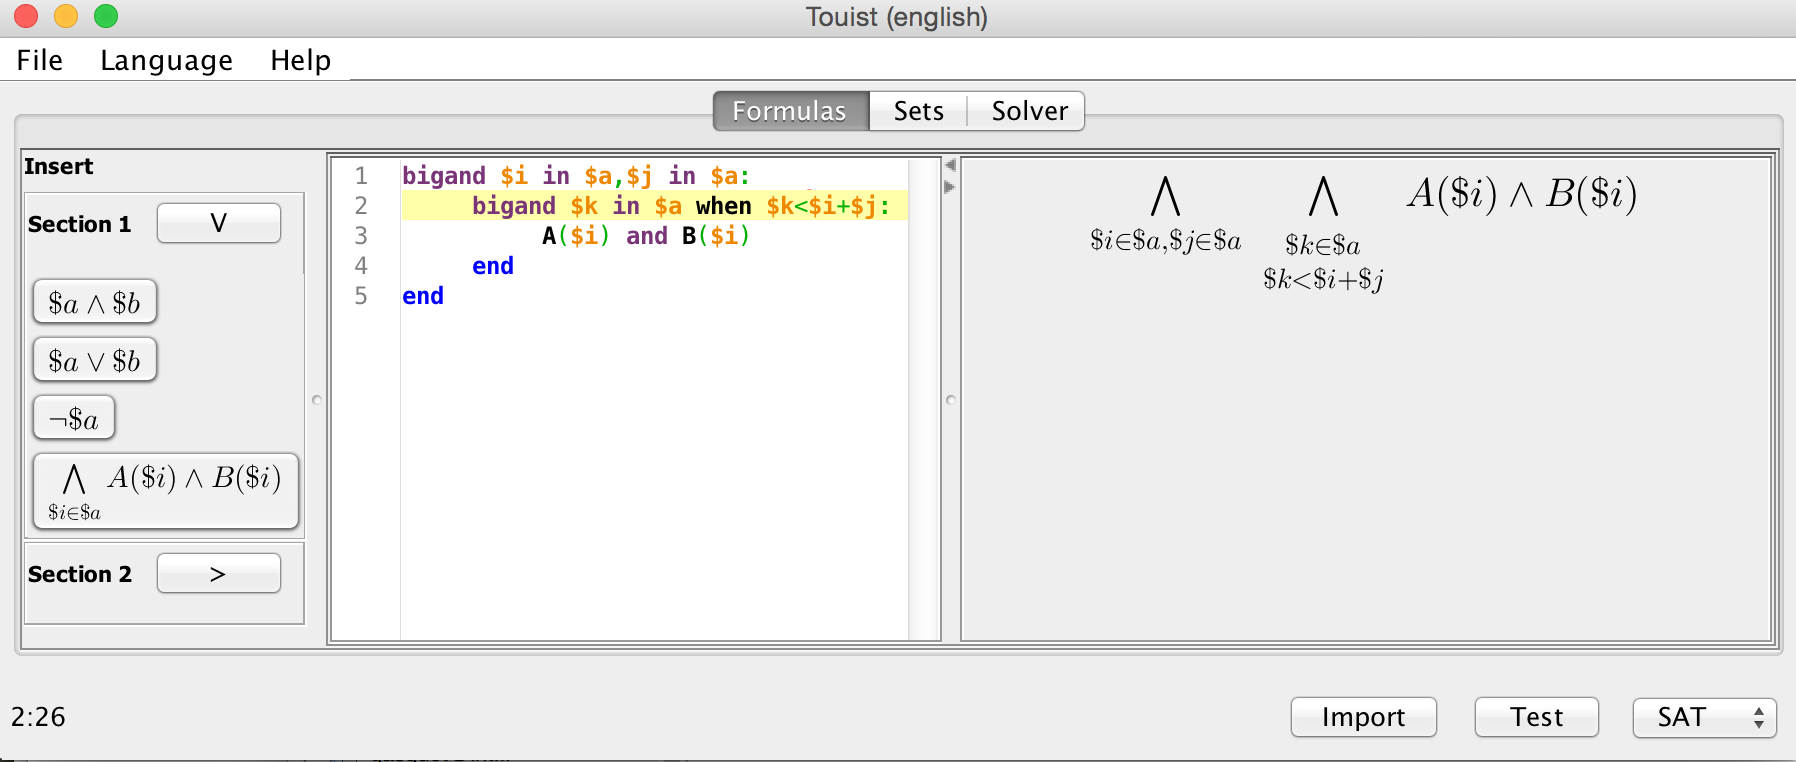
\includegraphics[scale=0.45]{LatexDisplay.png}
  \caption{Affichage en style \LaTeX}
  \label{fig:LatexDisplay}
\end{figure*}


En outre, les formules peuvent \^etre tap\'ees \`a la main dans la fen\^etre d'\'edition, ou introduites dans une sorte d'\'editeur dirig\'e par la syntaxe, en raffinant progressivement l'arbre syntaxique, ou encore elles peuvent \^etre import\'ees \`a partir d'un fichier externe.





%\begin{figure*}[ht]
%  \centering
%  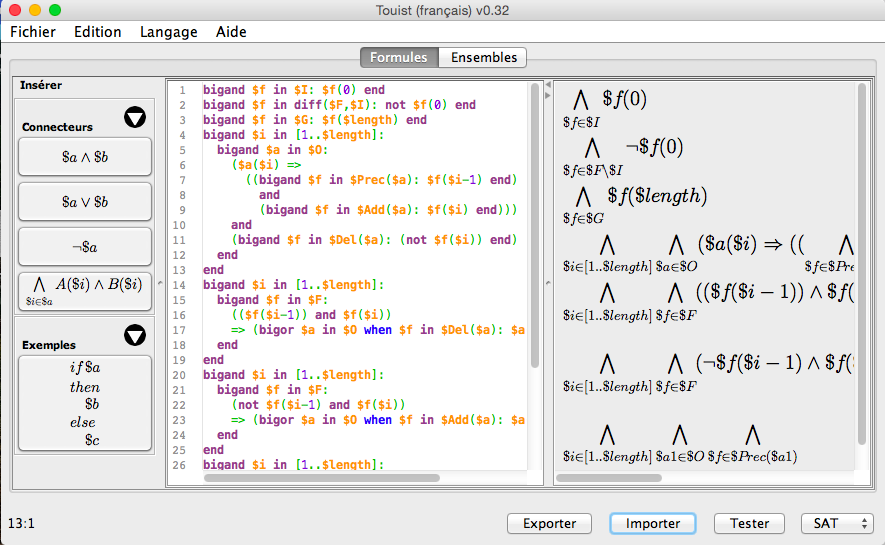
\includegraphics[scale=.4]{touist1.png}
%  \caption{Interface de TouIST}
%  \label{fig:touist}
%\end{figure*}






%%......................................................................
%\section{Behind the scenes}\label{sec:sat_behind}
%
%% !TeX root = IAF2015-TouIST.tex
% la ligne précédente sert pour le logiciel TexWorks afin de pouvoir compiler ce fichier directement sans devoir ouvrir satoulouse_main.tex!
The piece of software \satoulouse is an open-source project globally written in
JAVA so that it can be used on many different platforms.

\subsection{The graphical user interface}


The graphical user interface (GUI) enables the user to write formulas and to
click on the button ``check if the set of formulas is satisfiable''. The GUI
is written in JAVA in order to be able to use the suitable library SWING. In
particular, as this library is object oriented, it was really simple to create
our own widget to enter a formula of propositional logic. Formulas are also
displayed in \LaTeX\ style thanks to the library jLatexMath\footnote{\url{http://forge.scilab.org/index.php/p/jlatexmath/}} which does not require any
additional software (in particular it does not require a real \LaTeX\
installation).


\subsection{The SAT solver}

The SAT solver used as backend of \satoulouse\ is SAT4J
\footnote{\url{http://www.sat4j.org/}}. The first advantage of this solver is
that it is written in JAVA so it is easy to call it from the GUI. The second
one is its good efficiency \cite{berre10:_sat4j}, and even if it is not the best SAT
solver in the world (see SAT Race 2008), it is one of the best. 


\subsection{Connection between the SAT solver and the graphical user interface}

The translation from formulas written by the user to formulas for the SAT
solver SAT4J is divided in two parts:
\begin{itemize}
\item expanding formulas, that is to say, rewrite macros into expanded
  conjunction normal forms. For instance, we expand the formula $\bigwedge_{i
    \in \{1 .. 4\}} p_i$ into $(((p_1 \land p_2) \land p_3) \land
  p_4)$. Expanding formulas is done in Scheme code intepreted with the JAVA
  library kawa \cite{bothner1998kawa}. Scheme is a suitable language to
  perform this translation because parsing of formulas is directly done in
  this language: formulas are directly s-expressions.

\item translating the expanded conjunctive normal forms into a rigorous SAT4J
  input. This part is done in Java because we need to run SAT4J which is coded
  in JAVA. We construct a map between the propositions of the GUI (strings)
  and strict positive integers used by SAT4J and then build corresponding
  arrays of integer for SAT4J.
\end{itemize}



\subsection{Loading and saving a problem}

As we can give explicit names to propositions (and not only integers as for
SAT4J), as we have macros (like $\bigwedge_{i \in \{1 .. 4\}} switch_i$),
\satoulouse\ has its own file format: we simply write s-expressions representing
formulas. Nevertheless, \satoulouse\ is also able to load standard DIMACS cnf
format files as depicted below.\\[0pt]


%\begin{figure}
%\begin{center}
\begin{minipage}{6cm}
\begin{center}
\begin{verbatim}
c A sample .cnf file. 
p cnf 3 2
1 -3 0
2 3 -1 0 
1 2 -3 0
\end{verbatim}
\end{center}
\end{minipage}
\begin{minipage}{6cm}
\mbox{  }\\[18pt]
$((p_1 \vee \neg p_3) \wedge$

$(p_2 \vee p_3 \vee \neg p_1) \wedge$

$ (p_1 \vee p_2 \vee \neg p_3))$s
\end{minipage}
%\end{center}
%\caption{
\begin{center}The standard DIMACS cnf format\label{figure:dimacsformat}\end{center}
%}
%\end{figure}

%\begin{figure}
%%\begin{center}
%\begin{tabular}{lll}
%%\begin{center}
%%\begin{verbatim}
% c A sample .cnf file. & &\\
%p cnf 3 2 & \\
%1 -3 0  & \phantom{xxxxxxxxxxxxxxx} & $((p_1 \vee \neg p_3) \wedge$ \\
%2 3 -1 0  & & $(p_2 \vee p_3 \vee \neg p_1) \wedge$\\
%1 2 -3 0 & & $ (p_1 \vee p_2 \vee \neg p_3))$
%%\end{verbatim}
%%\end{center}
%\end{tabular}
%\caption{The standard DIMACS cnf format\label{figure:dimacsformat}}
%\end{figure}

%%% Local Variables: 
%%% mode: latex
%%% TeX-master: "satoulouse_main"
%%% End: 

%

%......................................................................
\section{Sujets avanc\'es pour les \'etudiants de cycles sup\'erieurs}\label{sec:advanced_topics}
%......................................................................


Dans ce qui suit, nous pr\'esentons tr\`es succictement quelques fonctionnalit\'es avanc\'ees de \nameTool. Elles devraient int\'eresser les \'etudiants de cycles sup\'erieurs et leurs enseignants bien s\^ur. Elles concernent SMT (SAT Modulo Theories), la planification par satisfaction de base de clauses (planification SAT) et leur combinaison la planification SMT.


\subsection{SMT: SAT Modulo Theories}

Certains probl\`emes combinatoires n\'ecessitent n\'eanmoins de traiter des calculs sur les nombre naturels ou r\'eels. Ceci peut \^etre fait en utilisant seulement la logique propositionnelle (par exemple, $2+3=5$ pourrait \^etre cod\'e par $add_{2,3,5}$), mais c'est tr\`es inconfortable \`a moins qu'il n'y ait que quelques additions \`a faire. Ne parlons m\^eme pas des op\'erations de multiplication ou plus complexes. L'id\'ee derri\`ere la gen\`ese de SMT a \'et\'e de combiner des solveurs SAT avec un solveur arithm\'etique dans le but d'am\'eliorer le traitement de la partie arithm\'etique du raisonnement. Dans de nombreux cas, ceci n'am\'eliorera pas seulement l'efficacit\'e du solveur, mais permettra aussi d'exprimer les contraintes arithm\'etiques des probl\`emes d'une mani\`ere radicalement plus compacte.

Pensez au jeu de Kamaji\footnote{\texttt{http://fr.wikipedia.org/wiki/Kamaji}}  o\`u le joueur doit grouper des nombres adjacents dans une grille de sorte que leur somme soit \'egale \`a un nombre fixe. R\'esoudre le jeu n\'ecessite essentiellement un raisonnement logique mais a aussi besoin d'un peu d'arithm\'etique (addition).


Si $x_{i,j}$ pour chaque case $(i,j)$ est un entier et $G(i,j,i,k)$ repr\'esente le fait que les cases $(i,j)$ \`a $(i,k)$ de la ligne $i$ forment un groupe, la contrainte de somme pourrait \^etre exprim\'ee par :
$$\sum_{m\in E}x_{i,m}=N$$
o\`u $N$ est le nombre fixe et $E$ est $\{j,j+1,\ldots,k\}$. La logique propositionnelle pure n'est certainement pas adapt\'ee pour de telles phrases !




\subsection{\nameTool\ pour la planification classique SAT}

En Intelligence Artificielle, la \emph{planification} est un processus cognitif qui consiste \`a g\'en\'erer automatiquement, au travers d'une proc\'edure formelle, un r\'esultat articul\'e sous la forme d'un syst\`eme de d\'ecision int\'egr\'e appel\'e \emph{plan}. Le plan est g\'en\'eralement sous la forme d'une collection organis\'ee d'\emph{actions} et il doit permettre \`a l'univers d'\'evoluer de l'\emph{\'etat initial} \`a un \'etat qui satisfait le \emph{but}. Dans le cadre classique, le plus restrictif, on consid\`{e}re les actions comme des transitions instantan\'{e}es sans prendre en compte le temps.

La planification par satisfaction de base de clauses (planification SAT) a \'et\'e introduite avec le planificateur SATPLAN \cite{kautzS92_planning_sat}. Dans cette approche, on travaille directement sur un ensemble fini de variables propositionnelles. Deux actions identiques pouvant appara\^{i}tre \`a des endroits diff\'erents d'un m\^{e}me plan doivent pouvoir \^{e}tre diff\'{e}renci\'{e}es et on leur associe donc des propositions diff\'erentes. Comme on ne conna\^{i}t pas \`a l'avance la longueur d'un plan solution d'un probl\`eme, on ne peut pas cr\'eer un codage unique permettant de le r\'esoudre puisqu'il faudrait cr\'eer une infinit\'e de variables propositionnelles pour repr\'esenter toutes les actions de tous les plans possibles. La solution la plus commune consiste alors \`a cr\'eer un codage repr\'esentant tous les plans d'une longueur $k$ fix\'ee. La base de clause ainsi obtenue est donn\'ee en entr\'ee \`a un solveur SAT qui retourne, lorsqu'il existe, un mod\`ele de cette base. Le d\'ecodage de ce mod\`ele permet alors d'obtenir un plan-solution. Si la r\'esolution du codage ne donne pas de mod\`ele, la valeur de $k$ est augment\'ee et le processus r\'eit\'er\'e. Pour la compl\'etude du proc\'ed\'e, tous ces mod\`eles doivent correspondre exactement \`a tous les plans solutions d'une longueur fix\'ee du probl\`eme.


Une diff\'erence importante de \nameTool\, en comparaison avec \satoulouse\, est sa capacit\'e \`a prendre en compte \`a la fois des formules logiques et ensembles de domaines. Par exemple, si l'on veut r\'esoudre un probl\`eme de planification particulier, \satoulouse\ est facile \`a utiliser pour d\'ecrire le probl\`eme et le r\'esoudre via un solveur SAT. Mais si notre objectif est de r\'esoudre plusieurs probl\`emes de planification g\'en\'eriques, nous pouvons profiter de la flexibilit\'e de \nameTool\ qui permet \`a l'utilisateur de d\'ecrire une m\'ethode g\'en\'erique de r\'esolution avec des r\`egles encod\'ees comme formules et d'utiliser des ensembles de domaines pour d\'ecrire chaque probl\`eme de planification particulier. De nombreuses r\`egles de codage pour la r\'esolution de probl\`emes de planification ont d\'ej\`a \'et\'e propos\'ees \cite{kautzS92_planning_sat,MaliK99_plan_space_encodings,Rintanen:2006}. Comme exemple d'une telle r\`egle nous donnons ci-apr\`es un codage des \emph{frame-axioms}. Si un fait est faux \`a une \'etape $i-1$ d'un plan solution et devient vrai \`a l'\'etape $i$, alors la disjonction des actions qui peuvent \'etablir le fait \`a l'\'etape $i$ du plan est vraie. C'est \`a dire, au moins une action qui \'etablit le fait doit avoir \'et\'e appliqu\'ee.


  \[\begin{aligned}\bigwedge_{i\in\{1..longueur\_plan\}}
  \bigwedge_{f\in Faits} \hspace{4cm}\\
  \left((\lnot f(i-1) \wedge f(i)) \Rightarrow 
  \bigvee_{a\in Actions / f\in Effets(a)} a(i)\right)\end{aligned}\]
\\


\subsection{\nameTool\ pour la planification temporelle SMT}

Pour r\'esoudre des probl\`emes de planification r\'eels, l'une des principales difficult\'es \`a surmonter consiste \`a prendre en compte la dimension temporelle. En effet, de nombreux probl\`emes du monde r\'eel n\'ecessitent, pour \^{e}tre r\'esolus ou ex\'ecut\'es plus efficacement, la prise en compte de la dur\'ee des actions, des instants auxquels des \'ev\`enements se produisent, ou encore la concurrence d'actions.

En compl\'ement de SAT, notre nouvelle plateforme \nameTool\ est capable de g\'erer des th\'eories comme la diff\'erence logique ou l'arithm\'etique lin\'eaire sur les nombres entiers (QF\_IDL, QF\_LIA) ou les nombres r\'eels (QF\_RDL, QF\_LRA), et d'appeler un solveur SMT pour trouver une solution. Pour \^etre r\'esolus, les probl\`emes de planification temporelle issus du monde r\'eel n\'ecessitent une repr\'esentation continue du temps, et donc, l'utilisation de nombres r\'eels dans les codages logiques. \nameTool\ peut \^etre utilis\'e pour r\'esoudre de tels probl\`emes impliquant des actions avec dur\'ee, des \'ev\`enements exog\`enes et des buts temporellement \'etendus, par exemple avec les r\`egles de codage propos\'ees dans \cite{MarisRegnier08}. Nous donnons ci-apr\`es un codage des exclusions mutuelles temporelles d'actions. Si deux actions $a$ et $b$ produisant respectivement une proposition $p$ et sa n\'egation sont actives dans le plan ($a \wedge b$ est vrai), alors l'intervalle de temps $[\tau(a \mid\rightarrow p), \tau(a \rightarrow\mid p)]$ correspondant \`a l'activation de $p$, et l'intervalle de temps $[\tau(b \mid\rightarrow \lnot p), \tau(b \rightarrow\mid \lnot p)]$ correspondant \`a l'activation de $\NOT p$ sont disjoints. Dans ce cas, il faut ajouter une disjonction pour imposer que la fin de l'un de ces intervalles soit strictement avant le d\'ebut de l'autre.

  \[\bigwedge_{a\in Actions}
  \bigwedge_{b\in Actions}
  \bigwedge_{f\in Faits | f\in Effets(a) \wedge \lnot f\in Effets(b)}\]
  \[\left(\left(a \wedge b\right) \Rightarrow 
  \left( \begin{aligned} \left(\tau(b \rightarrow\mid \lnot f) < \tau(a \mid\rightarrow f)\right)
    \\ \vee
    \left(\tau(a \rightarrow\mid f) < \tau(b \mid\rightarrow \lnot f)\right)
 \end{aligned} \right)\right) \]






%----------------------------------------------------------------------

%\vspace{-1cm}
\section{Conclusion}\label{sec:evaluation}

A notre connaissance, il n'existe pas d'autre outil qui cible un public aussi large, ni la m\^eme grande classe de probl\`emes, ni avec le m\^eme confort d'utilisation. La plupart des outils p\'edagogiques existants (soit l'impl\'ementation de tables de v\'erit\'e ou tableaux s\'emantiques) qui pourraient faire le travail de recherche d'un mod\`ele ne peuvent pas g\'erer efficacement de gros prob\`emes, et de vrais outils capables de les traiter ne sont cetainement pas con\c cus pour \^etre utilis\'es par des d\'ebutants en logique, et m\^eme pas par la plupart des \'etudiants de cycles sup\'erieurs.
Des outils avanc\'es con\c cus pour des sujets d'\'etudes sup\'erieures, comme Mozart \cite{DBLP:conf/moz/2004} ou Alloy  \cite{Jackson:2006:SAL:1146359} ont une courbe d'apprentissage raide qui peut dissuader les d\'ebutants et les utilisateurs non-sp\'ecialistes.

Nous croyons que \nameTool\ sera utile pour les d\'ebutants en logique ainsi que pour les utilisateurs avanc\'es gr\^{a}ce \`a sa grande gamme d'applications et sa facilit\'e d'utilisation.




% Bibliographie en utilisant BibTeX
\bibliography{IAF2015-TouIST}



\end{document}
